\documentclass{article}
\usepackage[margin=1.00in]{geometry}
\usepackage{listings}
\usepackage{graphicx}
\usepackage{amsmath}
\title{Analysis of Heuristic and Non-Heuristic Approaches to Classical Planning in Project \#3}
\author{Steven Bogacz}
\date{September 2017}
\begin{document}
\maketitle
\begin{section}{Problems}
\begin{subsection}{Problem \#1}
	\begin{subsubsection}{Initial State and Goal}
	\begin{verbatim}
	Init(At(C1, SFO) ∧ At(C2, JFK) 
	∧ At(P1, SFO) ∧ At(P2, JFK) 
	∧ Cargo(C1) ∧ Cargo(C2) 
	∧ Plane(P1) ∧ Plane(P2)
	∧ Airport(JFK) ∧ Airport(SFO))
Goal(At(C1, JFK) ∧ At(C2, SFO))\end{verbatim}
\end{subsubsection}
\begin{subsubsection}{Solution}
	\begin{verbatim}
		Load(C1, P1, SFO)
		Fly(P1, SFO, JFK)
		Load(C2, P2, JFK)
		Fly(P2, JFK, SFO)
		Unload(C1, P1, JFK)
		Unload(C2, P2, SFO)
	\end{verbatim}
\end{subsubsection}
\end{subsection}
\begin{subsection}{Problem \#2}
	\begin{subsubsection}{Initial State and Goal}
	\begin{verbatim}
Init(At(C1, SFO) ∧ At(C2, JFK) ∧ At(C3, ATL) 
		∧ At(P1, SFO) ∧ At(P2, JFK) ∧ At(P3, ATL) 
		∧ Cargo(C1) ∧ Cargo(C2) ∧ Cargo(C3)
		∧ Plane(P1) ∧ Plane(P2) ∧ Plane(P3)
		∧ Airport(JFK) ∧ Airport(SFO) ∧ Airport(ATL))
Goal(At(C1, JFK) ∧ At(C2, SFO) ∧ At(C3, SFO))\end{verbatim}
\end{subsubsection}
\begin{subsubsection}{Solution}
	\begin{verbatim}
Load(C1, P1, SFO)
Fly(P1, SFO, JFK)
Load(C2, P2, JFK)
Fly(P2, JFK, SFO)
Load(C3, P3, ATL)
Fly(P3, ATL, SFO)
Unload(C3, P3, SFO)
Unload(C1, P1, JFK)
Unload(C2, P2, SFO)
	\end{verbatim}
\end{subsubsection}
\end{subsection}
\begin{subsection}{Problem \#3}
	\begin{subsubsection}{Initial State and Goal}
	\begin{verbatim}
Init(At(C1, SFO) ∧ At(C2, JFK) ∧ At(C3, ATL) ∧ At(C4, ORD) 
		∧ At(P1, SFO) ∧ At(P2, JFK) 
		∧ Cargo(C1) ∧ Cargo(C2) ∧ Cargo(C3) ∧ Cargo(C4)
		∧ Plane(P1) ∧ Plane(P2)
		∧ Airport(JFK) ∧ Airport(SFO) ∧ Airport(ATL) ∧ Airport(ORD))
Goal(At(C1, JFK) ∧ At(C3, JFK) ∧ At(C2, SFO) ∧ At(C4, SFO))
\end{verbatim}
\end{subsubsection}
\begin{subsubsection}{Solution}
	\begin{verbatim}
Load(C2, P2, JFK)
Fly(P2, JFK, ORD)
Load(C4, P2, ORD)
Fly(P2, ORD, SFO)
Load(C1, P1, SFO)
Fly(P1, SFO, ATL)
Load(C3, P1, ATL)
Fly(P1, ATL, JFK)
Unload(C4, P2, SFO)
Unload(C3, P1, JFK)
Unload(C1, P1, JFK)
Unload(C2, P2, SFO)
	\end{verbatim}
\end{subsubsection}
\end{subsection}
\end{section}
\begin{section}{Comparing and Contrasting Search Metrics}
	The comprehensive metrics collected over the course of this project are shown below. I made an effort to
	collect metrics for every combination of problem and search method, however, excessive runtime prevented me from exhausting
	every combination. Those that were unable to run within a reasonable time frame are marked as "N/A".\par
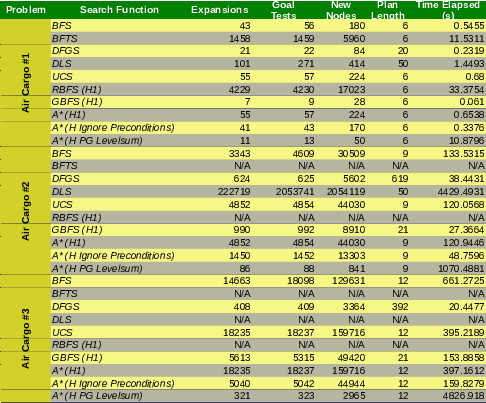
\includegraphics[width=\textwidth]{heuristics}
\begin{subsection}{Non-heuristic Search Result Comparison}
	In this project we used 5 different non-heuristic search methods (with their respective abbreviations listed parenthetically):
	\begin{itemize}
		\item Breadth First Search (BFS)
		\item Breadth First Tree Search (BFTS) 
		\item Depth First Graph Search (DFS)
		\item Depth Limited Search (DLS)
		\item Uniform Cost Search (UCS)
	\end{itemize}
	Perhaps it is easier to discuss the search methods starting by those which are demnonstrably less efficient. Breadth First 
	tree search was one of the two search methods to fall over first (it failed to complete for both problems two and three). 
	Both it and Recursive Best First Search required disproportionately more node expansions than any other search method. Problem \#1 
	was the only one where heuristics could be collected for those two, and they expanded 13 and 42 times as many nodes as the next
	biggest expander (depth-limited search).\par
	
	Depth-limited search and Depth-First Graph Search both returned sub-optimal plans. On the other hand, Breadth-First Search and Uniform Cost Search
	not only completed for every test case, but they also involved the least expansions out of the other non-heuristic based search methods. BFS was 
	more computationaly expensive, taking more time on problems \#2 and \#3, while UCS took up more memory with more expansions, but took less time to
	arrive to a solution. 
\end{subsection}
\begin{subsection}{Heuristic Search Result Comparison}
	The five heuristic based search methods we used are listed below:
	\begin{itemize}
		\item Recursive Best First Search H 1 (RBFS)
		\item Greedy Best First Graph Search H 1 (GBFS)
		\item A* Search H 1 (A*)
		\item A* Search H Ignore Preconditions (A*)
		\item A* Search H PG Level Sum (A*)
	\end{itemize}
	RBFS was already discussed in the previous section, so I will focus on the other four methods here. Interestingly, all four were able to finish within 
	a reasonable time frame, although there are significant tradeoffs to be considered. Greedy Best First Search and A* with the Ignore Preconditions Heuristic
	were the two fastest methods. GBFS has a substantial edge for smaller state spaces, but that advantage dissipates rapidly as the state space grows.\par
	GBFS did not, however, find an optimal solution in the case of Problem \#3. A* using the Level Sum Heuristic took far longer to compute (about an order of
	magnitude) but also expanded far less nodes, by about a factor of ten. Ultimately, it seems that the trade-off would be situation dependent: are we more
	constrained by available computation time, or are we running in a memory-limited environment?\par

	Overall, the heuristic-based search methods were generally more performant than the non-heuristic based search methods. Even the Level Sum heuristic,
	despite having a significantly longer run time than the two optimal non-heuristic searches, BFS and UCS, came at a far lesser memory cost. A* with the
	Ignore Preconditions Heuristic not only arrived to the same optimal solution, but also did so in a quarter and half the time than each BFS and UCS 
	respectively. Looking at the trend, it seems clear that this outperformace would grow along with the size of the state space. 
\end{subsection}
\end{section}
\end{document}
